\documentclass[a4paper]{article}

\usepackage[T1]{fontenc}
\usepackage[utf8]{inputenc}
\usepackage{lmodern}

\usepackage[english]{babel}
\usepackage{csquotes}
\usepackage{graphicx}

\usepackage[notes,backend=biber]{biblatex-chicago}
\bibliography{sample}


\begin{document}

\centre{
\title{\Huge{Measuring Software Engineering \\ CSU33012}}
\author{\Large{Caroline \textsc{Liu}}}
\date{\large{7\textsuperscript{th} November }}
\maketitle
}
\clearpage
\large{
\tableofcontents

\clearpage

\section{Abstract}
This report discusses the ways in which the software engineering process can be measured and assessed in terms of measurable data, an overview of the computational platforms available to perform this work, the algorithmic approaches available and the ethical concerns surrounding this kind of analytics.

\section{Introduction}
The IEEE defines software engineering as:
\begin{itemize}
    \item The application of a systematic, disciplined, quantifiable approach to the development,operation and maintenance of software; that is, the application of engineering to software.
    \item The study of approaches as in the above statement.\autocite{R01}
\end{itemize}
In summary, software engineering is the development of software fulfilling the users needs and thus using well-defined scientific principles, methods and procedures to execute the process.
\bigbreak
The main principles of software engineering include:
\begin{itemize}
    \item \textbf{Separation of concerns}: when specifying the details for the development of an application or its component, there are often two concerns that need to be encountered: basic functionality and support for data integrity. Run-time efficiency is a common example of this.
    \item \textbf{Modularity}: this is a specialisation of the above principle where its procedure is to separate the software components according to functionality and components.
    \item \textbf{Abstraction}:  this is another specialisation of the principle of separation of concerns. This requires for the developer to separate the components of the software from their implementation and considering them by functionality and implementation.
    \item \textbf{Anticipation of Change}: working out an automated solution is both a learning experience for the users and the developers. When problems arise, the users would expect the developers to come up with a reasonable solution as soon as possible. This would not only be a timely challenge, but also one that requires both the user and developer to be familiar in their own perspective about the program and the program itself to have been developed in such a manner that its components and other functionalities would not be prone to the changes being made.
    \item \textbf{Generality}: this is closely related to the principle of anticipation of change. This states that it is key when designing the software to ensure that it is free from unnatural restrictions and limitations. An example of this is the two digit formatting of year numbers, which lead to the "year 2000" problem. Users learn their actual needs when they see the gradual development of the program.
    \item \textbf{Incremental Development}: this is a method that aids in simplifying the process of software development by only considering rigid testing on the incremental component added to the software at each stage until the projected functionalities are fulfilled.
    \item \textbf{Consistency}: this is a principle is a recognition of the fact that it is easier to do things in familiar context serving both the user and the software engineer for future improvements. Coding style is an example of this.\autocite{R02}
\end{itemize}

\section{History of Software Engineering}
Digital computers first appeared in the early 1940s, the instructions to make them operate were wired into the machine.\autocite{R03} This aided the discovery of the von Neumann architecture of computers. This gradually lead to the establishment the division between hardware and software as the complexity of abstraction being used to deal with computing. 
\bigbreak
Then came the development of programming languages in the early 1950s such as Fortran, ALGOL, and COBOL to deal with real world problems. Shortly after this, cam the \textit{software crisis} of the 1960s, 1970s, and 1980s, this caused the stimulated the development of software engineering in which some fundamental problems a the times were identified. These included concepts such as:
\begin{itemize}
    \item Cost and budget overturns
    \item Property damage
    \item Life and death\autocite{R04}
\end{itemize}
\bigbreak
During the 1960s, writing software has evolved into finding the best ways to maximise the quality of software and methods in the building it. Quality can refer to how maintainable software is, to its stability, speed usability, testability, readability, size, cost, security and number of flaws, as well as many more attributes.
\bigbreak
Peter G. Neumann has kept a contemporary list of software problems and disasters.\autocite{R05} The crisis gradually faded from view due to the prolonged period of the instance. Michael A. Jackson has written extensively about the nature of software engineering\autocite{R06}, framing the problems that whether software engineering is to become an engineering science. During this period also, David Parnas introduced two of the the main concept of software engineering: modularity and data integrity in 1972.
\bigbreak
For decades, solving the software crisis was at most importance for researchers and companies producing software tools. The cost of owning software was the burden of the time.
\bigbreak
Every new technology and practice including tools, discipline, formal methods, process and professionalism, from the 1970s through the 1990s was seem as a \textit{silver bullet} to solve the software crisis. Though in 1986, an article titled "No Silver Bullet" was published by Fred Books, stating the argument that "\textit{there is no single development, in either technology or management technique which by itself promises even one order of magnitude (tenfold) improvement within a decade in productivity, in reliability, in simplicity}."\autocite{R07}
\bigbreak
In 1984, the Software Engineering Institute was established and the SEI Software Process Program was founded and aimed at understanding and managing the software engineering process.
\bigbreak
As of today, these components have joint together enabling us to form a more precise understanding of the term software engineering, also allowing us to have a more identified process when developing software.

\section{Measurable Data}
Today, data is a way for software engineers to keep track of their delivered processes and keep up with the accelerated industry. Software metrics is a standard way of measuring many activities of production, which include the following:
\begin{itemize}
    \item \textbf{Product metrics}: which describe the characteristics of the products, including size, complexity, design features, and quality level.
    \item \textbf{Process metrics}: this data can be used for future development and maintenance purposes of the program.
    \item \textbf{Project metrics}: this data describes the project characteristics and execution.\autocite{R04}
\end{itemize}
\bigbreak
The main concern for tracking software metrics is to make measurements easy to collect or it will not be done. The purpose of collecting such data is to aid the improvements that could be made to the development team for higher production of the team. Gathering of such data should not be a burden of the process. Therefore, taking it into consideration, software metrics should have the following characteristics:
\begin{itemize}
    \item Relevant and reliable
    \item Simple and computable
    \item Consistent and objective
    \item Independent of programming language or platforms
    \item cost-efficient
    \item Adaptable\autocite{R08}
\end{itemize}
\bigbreak
Hence, it is important that software development platforms that automatically track these metrics.
\bigbreak
\subsection{Agile Development Methodology}
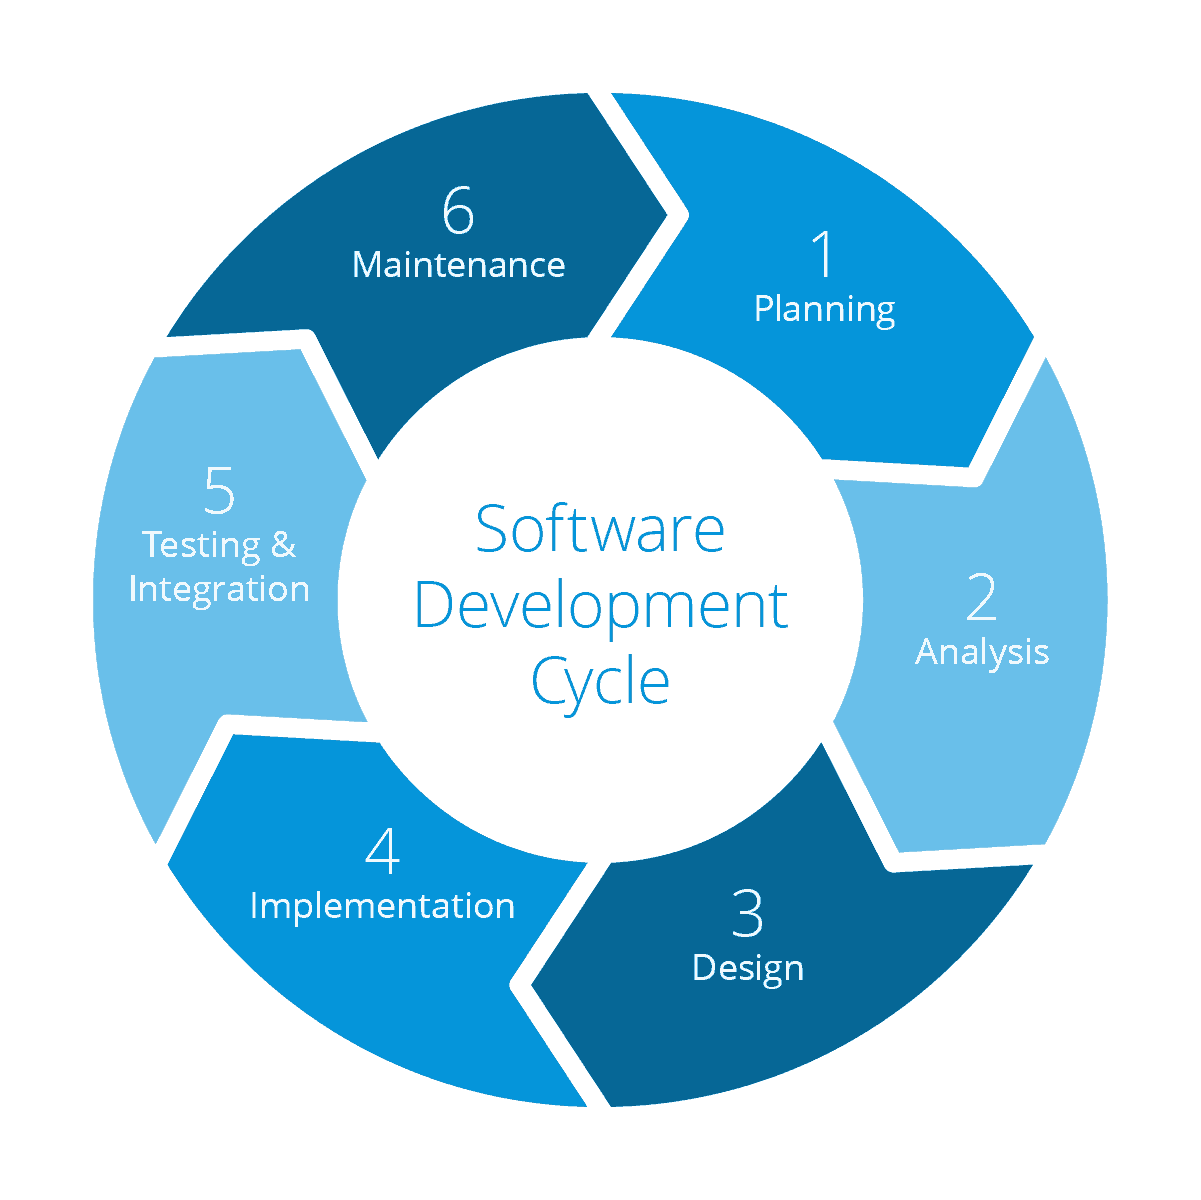
\includegraphics[scale = 0.2]{agile.png}
\autocite{D01}
\bigbreak
In agile methods, teams develop the software in iterations that contain mini-increments of the new functionality. This is more beneficial than betting everything all at once, but work is consumed in smaller units, robust testing would be done on the currently delivered work showing indications of improvements allowing restart of the mini-process, until the features and functionalities fulfill the current projections of the process. There are many different forms of the agile development method, including scrum, crystal, extreme programming (XP), and feature-driven development (FDD).
\bigbreak
Benefits of this type of development methodology is that it allows software to be released in iterations. Iterative improvements on the software would allow the team to identify problems at an early stage of the process an aid in the end quality of the deliverable product.
\bigbreak 
Agile, however, does have it's disadvantages including more time for the team invested into communication and more commitment required by the individual. It also has less predictability and would easily fail once the progress is off-track.

\subsection{Waterfall Method}
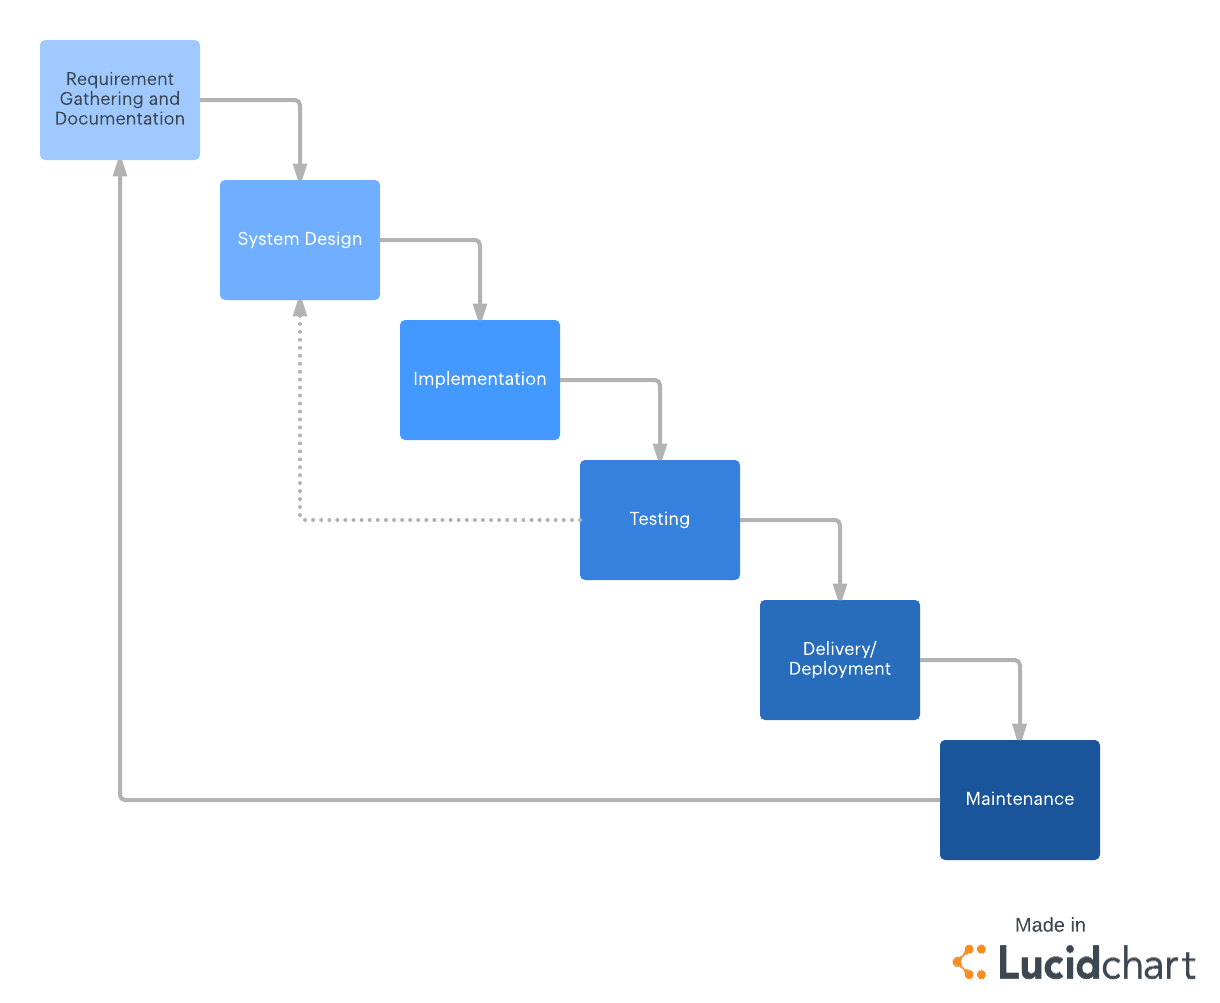
\includegraphics[scale=0.3]{waterfall.png}
\autocite{D02}
\bigbreak
Waterfall method is a rigid linear model that consists of sequential phases (requirements, design, implementation, verification, maintenance) focusing on distinct goals, which is the most traditional software development method. Each phase must be fully complete before proceeding. It is not quite flexible in that there is usually no process for backtracking previous phases.
\bigbreak
Benefits of this method include a clear, well defined structure of procedures and the clear set a stable goal from the initial stages of development. This make it easier to understand and manage the overall project.
\bigbreak
Disadvantages are obvious as this method does not allow for backtracking of processes, it is only when one stage is fully complete, that allows the team to move on to the next stage and delays testing.
\bigbreak

\subsection{Spiral Method}
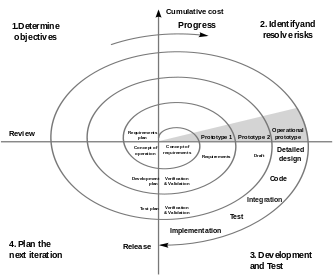
\includegraphics[scale=0.9]{spiral.png}
\autocite{D03}
\bigbreak
The spiral method adapts the spiral model, which is one of the most important software development life cycle model. It is graphically represented as infinite many loops on a spiral, the number of loops depend on the individual project. Each loop is called a phase of the process. It allows a more dynamical development of the project. The radius of the spiral at any point represent the expenses of the project and the angular dimension represents the progress made so far in the current phase.
\bigbreak
This method is good for large project and allows for risk analysis and risk handling at every phase. Changes in the requirements are allowed in later phases of the process and can be incorporated accurately by using this method.
\bigbreak
This method is much more complex than others and costly, therefore not suitable for small project. It is also too much dependable on risk analysis, without very highly experienced expertise, it is going to cause failure in the process. Management in time is also an issue as the time consumed by each phase at the initial stage of the project is unknown.

\subsection{Benefits of Tracking and Analysing Software Metrics}
Benefits of tracking and analysing software metrics is to determine the quality of the current product or process, and give an indication of the possible improvements that can be made to the software project, thus measure the quality of the overall completed project. This also aids the productivity in the workplace, for instance, managers would be able view this data and identify, prioritise, track and communicate or any other issues that can be resolved, benefiting the production levels.

\section{Computational Platforms}
Computational Platforms allows the above development methods to be assessed and software to be executed. Computing platforms have different abstraction levels, including a computer architecture, an OS, or run-time libraries.\autocite{R09} A platform can be seen as a constraint but also assure better code qualities and find "bugs" and aid the developer to find better solutions. The process in reviewing code could be time consuming but allows for better quality code.
\bigbreak
Platforms serve various purposes including allowing for automated execution of code, collaboration and development on cloud servers.

\subsection{Cloud Server}
Most services run off servers as opposed to personal computers, therefore there are platforms and tools built to deploy and execute the scripts and maintain the server. Examples of these include Docker, Microsoft Azure and Google Compute Engine.
\subsection{Collaboration and Integrity Checking}
The main output of the process of software engineering is the deliverable product. Nowadays, projects are often based on teams, and therefore require a collaboration platform for developing methods such as agile to work out. Platforms such as Github allow individuals to work by themselves and eventually merge their work into the main project, whilst also keeping backup and tracking their work. Features of such platforms are far more than this.

\section{Algorithmic Approaches}
There are various ways to measure and analyse the software engineering process. One of the most effective ways would be to use machine learning as it allows the process to develop for itself a set of test and rules dynamically.
\bigbreak
\subsection{Machine Learning}
Machine Learning defined by Tom Mitchell in 1998, is a well posed learning problem where a computer program is said to learn from the experience E, with respect to some task T and some performance measure P, if its performance on T, as measured by P, improves with experience E.\autocite{R11}
\bigbreak
Machine learning today, unlike the past, enable the program to learn from previous computations to produce reliable, repeatable decisions and results rather than before, where it initialised as pattern recognition and the theory that computers can learn without being programmed to perform specific tasks.\autocite{R10} Widely publicised examples of machine learning would include the following:
\begin{itemize}
    \item The self-driving Google car
    \item Amazon/Netflix recommendations
    \item Analysing customer reviews on social media
    \item Fraud detection
\end{itemize}
\bigbreak
Machine learning is important important as of today, data is of the essence. Analysis and automation of theses analyses to deliver faster and more accurate results allow companies to gain insights into their own performance against others of similar functionalities in the industry.
\bigbreak
Here are some of the various types of machine learning:
\subsubsection{Supervised Learning}
These types of algorithms are trained with the "right answers" given. These algorithms mainly deal with regression problems, where it is to predict continuous valued output, and classification in which the output is discrete i.e. yes or no.
\subsubsection{Unsupervised Learning}
Theses algorithms are trained without telling it the "correct" answer. It itself must analyse the data and find some sort of structure within. These algorithms are catagorised into two parts: clustering, where the aim is to discover the inherent groups of data, and association, where the aim is to discover rules that describe large portions of the data.
\subsubsection{Semi-supervised Learning}
These types of algorithms fall in between unsupervised and supervised learning. It typically takes in a small amount of labeled data with a large amount of unlabeled data, which study has shown it improves the learning accuracy.
\subsubsection{Reinforcement Learning}
This is an area where is it mainly about taking suitable actions to minimise rewards in a particular situation, which are often seen in gaming, robotics and navigation areas. The training of these algorithms are based upon the input (the initial state of the model) and the user will decide to reward or punish the model base on the output. The learning proceeds and the optimal solution is decided based on the maximum reward.\autocite{R12}

\section{Ethical Concerns}
Ethical issues occur when a given decision, scenario or activity creates a conflict with society's moral principles. Software engineers are to respect and be aware of the ethical concerns that may arise from their code and actions in the workplace. 
Some of the ethical issues in software engineering include:
\begin{itemize}
    \item \textbf{Privacy}: handling, storing, sharing user data only under circumstances and purposes that the user agrees to
    \item \textbf{Transparency}: transparent decision-making procedures in intelligent systems, publicly available ethics policies by software development organisations.
    \item \textbf{Diversity}: gender, race, and age distribution of professionals in a development team
    \item \textbf{Common Goods}: contributing to, using, promoting open source software
    \item \textbf{Work Ethics}: decisions on the priority of implementations of requests before the product is released
    \item \textbf{Accountability}: deciding the responsibility when flaws occur\autocite{R13}
\end{itemize}
\bigbreak
A fine example would be the General Data Protection Regulations, GDPR, brought out to give EU citizens more control over the their personal data. The aim is that both the individuals and companies would benefit, as companies must measure their performance under a legal basis.\autocite{R14}
\bigbreak 
It is hard to measure the rights and wrongs on tracking data as to the different ethical limits for different societies and individuals. It is certain that there is still a long way to go as to agreeing upon these regulations.
\bigbreak
\section{Conclusion}
This report discusses the various ways of measuring and assessing the process of software engineering with the components of measurable data, computational platforms, algorithmic approaches and ethical issues, that all aid the process to become more efficient and society-friendly.
}


\printbibliography

\end{document}